% Options for packages loaded elsewhere
\PassOptionsToPackage{unicode}{hyperref}
\PassOptionsToPackage{hyphens}{url}
\PassOptionsToPackage{dvipsnames,svgnames,x11names}{xcolor}
%
\documentclass[
  letterpaper,
  DIV=11,
  numbers=noendperiod]{scrartcl}

\usepackage{amsmath,amssymb}
\usepackage{iftex}
\ifPDFTeX
  \usepackage[T1]{fontenc}
  \usepackage[utf8]{inputenc}
  \usepackage{textcomp} % provide euro and other symbols
\else % if luatex or xetex
  \usepackage{unicode-math}
  \defaultfontfeatures{Scale=MatchLowercase}
  \defaultfontfeatures[\rmfamily]{Ligatures=TeX,Scale=1}
\fi
\usepackage{lmodern}
\ifPDFTeX\else  
    % xetex/luatex font selection
\fi
% Use upquote if available, for straight quotes in verbatim environments
\IfFileExists{upquote.sty}{\usepackage{upquote}}{}
\IfFileExists{microtype.sty}{% use microtype if available
  \usepackage[]{microtype}
  \UseMicrotypeSet[protrusion]{basicmath} % disable protrusion for tt fonts
}{}
\makeatletter
\@ifundefined{KOMAClassName}{% if non-KOMA class
  \IfFileExists{parskip.sty}{%
    \usepackage{parskip}
  }{% else
    \setlength{\parindent}{0pt}
    \setlength{\parskip}{6pt plus 2pt minus 1pt}}
}{% if KOMA class
  \KOMAoptions{parskip=half}}
\makeatother
\usepackage{xcolor}
\setlength{\emergencystretch}{3em} % prevent overfull lines
\setcounter{secnumdepth}{-\maxdimen} % remove section numbering
% Make \paragraph and \subparagraph free-standing
\makeatletter
\ifx\paragraph\undefined\else
  \let\oldparagraph\paragraph
  \renewcommand{\paragraph}{
    \@ifstar
      \xxxParagraphStar
      \xxxParagraphNoStar
  }
  \newcommand{\xxxParagraphStar}[1]{\oldparagraph*{#1}\mbox{}}
  \newcommand{\xxxParagraphNoStar}[1]{\oldparagraph{#1}\mbox{}}
\fi
\ifx\subparagraph\undefined\else
  \let\oldsubparagraph\subparagraph
  \renewcommand{\subparagraph}{
    \@ifstar
      \xxxSubParagraphStar
      \xxxSubParagraphNoStar
  }
  \newcommand{\xxxSubParagraphStar}[1]{\oldsubparagraph*{#1}\mbox{}}
  \newcommand{\xxxSubParagraphNoStar}[1]{\oldsubparagraph{#1}\mbox{}}
\fi
\makeatother

\usepackage{color}
\usepackage{fancyvrb}
\newcommand{\VerbBar}{|}
\newcommand{\VERB}{\Verb[commandchars=\\\{\}]}
\DefineVerbatimEnvironment{Highlighting}{Verbatim}{commandchars=\\\{\}}
% Add ',fontsize=\small' for more characters per line
\usepackage{framed}
\definecolor{shadecolor}{RGB}{241,243,245}
\newenvironment{Shaded}{\begin{snugshade}}{\end{snugshade}}
\newcommand{\AlertTok}[1]{\textcolor[rgb]{0.68,0.00,0.00}{#1}}
\newcommand{\AnnotationTok}[1]{\textcolor[rgb]{0.37,0.37,0.37}{#1}}
\newcommand{\AttributeTok}[1]{\textcolor[rgb]{0.40,0.45,0.13}{#1}}
\newcommand{\BaseNTok}[1]{\textcolor[rgb]{0.68,0.00,0.00}{#1}}
\newcommand{\BuiltInTok}[1]{\textcolor[rgb]{0.00,0.23,0.31}{#1}}
\newcommand{\CharTok}[1]{\textcolor[rgb]{0.13,0.47,0.30}{#1}}
\newcommand{\CommentTok}[1]{\textcolor[rgb]{0.37,0.37,0.37}{#1}}
\newcommand{\CommentVarTok}[1]{\textcolor[rgb]{0.37,0.37,0.37}{\textit{#1}}}
\newcommand{\ConstantTok}[1]{\textcolor[rgb]{0.56,0.35,0.01}{#1}}
\newcommand{\ControlFlowTok}[1]{\textcolor[rgb]{0.00,0.23,0.31}{\textbf{#1}}}
\newcommand{\DataTypeTok}[1]{\textcolor[rgb]{0.68,0.00,0.00}{#1}}
\newcommand{\DecValTok}[1]{\textcolor[rgb]{0.68,0.00,0.00}{#1}}
\newcommand{\DocumentationTok}[1]{\textcolor[rgb]{0.37,0.37,0.37}{\textit{#1}}}
\newcommand{\ErrorTok}[1]{\textcolor[rgb]{0.68,0.00,0.00}{#1}}
\newcommand{\ExtensionTok}[1]{\textcolor[rgb]{0.00,0.23,0.31}{#1}}
\newcommand{\FloatTok}[1]{\textcolor[rgb]{0.68,0.00,0.00}{#1}}
\newcommand{\FunctionTok}[1]{\textcolor[rgb]{0.28,0.35,0.67}{#1}}
\newcommand{\ImportTok}[1]{\textcolor[rgb]{0.00,0.46,0.62}{#1}}
\newcommand{\InformationTok}[1]{\textcolor[rgb]{0.37,0.37,0.37}{#1}}
\newcommand{\KeywordTok}[1]{\textcolor[rgb]{0.00,0.23,0.31}{\textbf{#1}}}
\newcommand{\NormalTok}[1]{\textcolor[rgb]{0.00,0.23,0.31}{#1}}
\newcommand{\OperatorTok}[1]{\textcolor[rgb]{0.37,0.37,0.37}{#1}}
\newcommand{\OtherTok}[1]{\textcolor[rgb]{0.00,0.23,0.31}{#1}}
\newcommand{\PreprocessorTok}[1]{\textcolor[rgb]{0.68,0.00,0.00}{#1}}
\newcommand{\RegionMarkerTok}[1]{\textcolor[rgb]{0.00,0.23,0.31}{#1}}
\newcommand{\SpecialCharTok}[1]{\textcolor[rgb]{0.37,0.37,0.37}{#1}}
\newcommand{\SpecialStringTok}[1]{\textcolor[rgb]{0.13,0.47,0.30}{#1}}
\newcommand{\StringTok}[1]{\textcolor[rgb]{0.13,0.47,0.30}{#1}}
\newcommand{\VariableTok}[1]{\textcolor[rgb]{0.07,0.07,0.07}{#1}}
\newcommand{\VerbatimStringTok}[1]{\textcolor[rgb]{0.13,0.47,0.30}{#1}}
\newcommand{\WarningTok}[1]{\textcolor[rgb]{0.37,0.37,0.37}{\textit{#1}}}

\providecommand{\tightlist}{%
  \setlength{\itemsep}{0pt}\setlength{\parskip}{0pt}}\usepackage{longtable,booktabs,array}
\usepackage{calc} % for calculating minipage widths
% Correct order of tables after \paragraph or \subparagraph
\usepackage{etoolbox}
\makeatletter
\patchcmd\longtable{\par}{\if@noskipsec\mbox{}\fi\par}{}{}
\makeatother
% Allow footnotes in longtable head/foot
\IfFileExists{footnotehyper.sty}{\usepackage{footnotehyper}}{\usepackage{footnote}}
\makesavenoteenv{longtable}
\usepackage{graphicx}
\makeatletter
\def\maxwidth{\ifdim\Gin@nat@width>\linewidth\linewidth\else\Gin@nat@width\fi}
\def\maxheight{\ifdim\Gin@nat@height>\textheight\textheight\else\Gin@nat@height\fi}
\makeatother
% Scale images if necessary, so that they will not overflow the page
% margins by default, and it is still possible to overwrite the defaults
% using explicit options in \includegraphics[width, height, ...]{}
\setkeys{Gin}{width=\maxwidth,height=\maxheight,keepaspectratio}
% Set default figure placement to htbp
\makeatletter
\def\fps@figure{htbp}
\makeatother

\KOMAoption{captions}{tableheading,figureheading}
\makeatletter
\@ifpackageloaded{tcolorbox}{}{\usepackage[skins,breakable]{tcolorbox}}
\@ifpackageloaded{fontawesome5}{}{\usepackage{fontawesome5}}
\definecolor{quarto-callout-color}{HTML}{909090}
\definecolor{quarto-callout-note-color}{HTML}{0758E5}
\definecolor{quarto-callout-important-color}{HTML}{CC1914}
\definecolor{quarto-callout-warning-color}{HTML}{EB9113}
\definecolor{quarto-callout-tip-color}{HTML}{00A047}
\definecolor{quarto-callout-caution-color}{HTML}{FC5300}
\definecolor{quarto-callout-color-frame}{HTML}{acacac}
\definecolor{quarto-callout-note-color-frame}{HTML}{4582ec}
\definecolor{quarto-callout-important-color-frame}{HTML}{d9534f}
\definecolor{quarto-callout-warning-color-frame}{HTML}{f0ad4e}
\definecolor{quarto-callout-tip-color-frame}{HTML}{02b875}
\definecolor{quarto-callout-caution-color-frame}{HTML}{fd7e14}
\makeatother
\makeatletter
\@ifpackageloaded{caption}{}{\usepackage{caption}}
\AtBeginDocument{%
\ifdefined\contentsname
  \renewcommand*\contentsname{Tabla de contenidos}
\else
  \newcommand\contentsname{Tabla de contenidos}
\fi
\ifdefined\listfigurename
  \renewcommand*\listfigurename{Listado de Figuras}
\else
  \newcommand\listfigurename{Listado de Figuras}
\fi
\ifdefined\listtablename
  \renewcommand*\listtablename{Listado de Tablas}
\else
  \newcommand\listtablename{Listado de Tablas}
\fi
\ifdefined\figurename
  \renewcommand*\figurename{Figura}
\else
  \newcommand\figurename{Figura}
\fi
\ifdefined\tablename
  \renewcommand*\tablename{Tabla}
\else
  \newcommand\tablename{Tabla}
\fi
}
\@ifpackageloaded{float}{}{\usepackage{float}}
\floatstyle{ruled}
\@ifundefined{c@chapter}{\newfloat{codelisting}{h}{lop}}{\newfloat{codelisting}{h}{lop}[chapter]}
\floatname{codelisting}{Listado}
\newcommand*\listoflistings{\listof{codelisting}{Listado de Listados}}
\makeatother
\makeatletter
\makeatother
\makeatletter
\@ifpackageloaded{caption}{}{\usepackage{caption}}
\@ifpackageloaded{subcaption}{}{\usepackage{subcaption}}
\makeatother
\ifLuaTeX
\usepackage[bidi=basic]{babel}
\else
\usepackage[bidi=default]{babel}
\fi
\babelprovide[main,import]{spanish}
% get rid of language-specific shorthands (see #6817):
\let\LanguageShortHands\languageshorthands
\def\languageshorthands#1{}
\ifLuaTeX
  \usepackage{selnolig}  % disable illegal ligatures
\fi
\usepackage{bookmark}

\IfFileExists{xurl.sty}{\usepackage{xurl}}{} % add URL line breaks if available
\urlstyle{same} % disable monospaced font for URLs
\hypersetup{
  pdftitle={Los primeros pasos},
  pdfauthor={Miguel Equihua},
  pdflang={es},
  colorlinks=true,
  linkcolor={blue},
  filecolor={Maroon},
  citecolor={Blue},
  urlcolor={Blue},
  pdfcreator={LaTeX via pandoc}}

\title{Los primeros pasos}
\author{Miguel Equihua}
\date{Xalapa, Ver., 21 de febrero, 2025}

\begin{document}
\maketitle

\subsection{\texorpdfstring{\href{https://rstudio.github.io/cheatsheets/quarto.pdf}{Markdown}
y la \href{pres-ciencia-abierta.qmd}{ciencia
abierta}}{Markdown y la ciencia abierta}}\label{markdown-y-la-ciencia-abierta}

\emph{Tan simple como escribir en la página en blanco con pequeñas
marcas de intención}. Se ha inventado varias veces y el columpio ha ido
y venido entre el interés en ver y controlar las marcas directamente
sobre el texto y la preferencia de ver sólo el producto terminado
\textbf{WYSIWYG} (\emph{lo que ves es lo que tienes}, aunque el marcado
existe, pero lo hace la máquina por ti).

\begin{figure}

\begin{minipage}{0.40\linewidth}
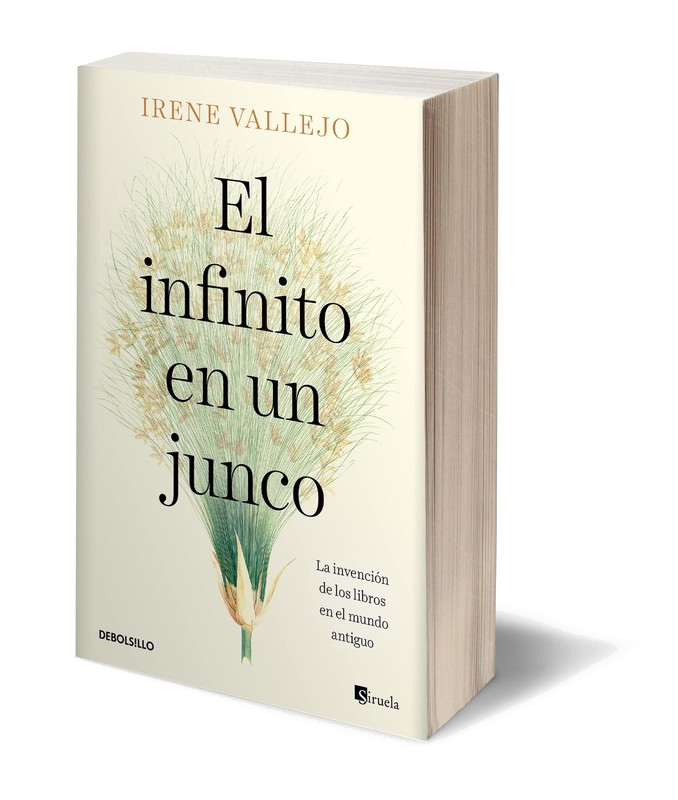
\includegraphics[width=2.08333in,height=\textheight]{images/900-el-infinito-en-un-junco-irene-vallejo-alfa.png}\end{minipage}%
%
\begin{minipage}{0.60\linewidth}
El trabajo del científico, el ingeniero, el estudiante o el creador de
contenidos transita por el proceso de escribir, almacenar y dar formato
presentable a los documentos. La escritura da origen a la historia y
deja atras la prehistoria. Un largo proceso de evolución cultural
apasionante que tiene un hermoso recuento en el libro de Irene Vallejo
\emph{El infinito en un Junco}. Hemos explorado las rocas, la arcilla,
los pigmentos vegetales y minerales, las pieles de animales y los
tejidos vegetales para escribir.\end{minipage}%

\end{figure}%

Hoy lo hacemos sobre el éter y nos apoyamos en procesos
electromagnéticos. Hacer esto ha involucrado a incontables inventores y
lo hacemos recurriendo a herramientas y formatos que tienen registro de
propiedad a nombre de lucrativas empresas particulares. Lo hacemos así y
el hecho no nos merece ni un suspiro reflexivo sobre sus implicaciones.

A veces nos incomodan detalles o grandes fallas que obstaculizan la
expresividad que requiere la escritura académica creativa. En general,
la práctica actual se opone a lograr un flujo ágil y transparente a lo
largo del proceso completo que involucra organizar los datos,
analizarlos, sintetizarlos y publicar los hallazgos obtenidos.

Por la fuerza del hábito, y a pesar de inconvenientes, la mayoría de las
revistas aún insisten en recibir textos en formato \textbf{docx}.

En el movimiento social que nos invita a reflexionar sobre la
\emph{ciencia abierta}, hay quienes sostenemos que el conocimiento y el
proceso creativo que lo impulsa debe ser lo más libre posible. El
talento y la sabiduría su núcleo. Sobre todo en áreas como la salud y la
calidad del entorno ecológico en el que vivimos.

\begin{figure}

\begin{minipage}{0.58\linewidth}
Markdown fue desarrollado en 2004 por \textbf{John Gruber}. Ideo una
manera de poner marcas de formato en un texto cómun y corriente (lo
llamaremos \emph{texto plano}). También construyó un programa de cómputo
(lo escribió en el lenguaje Perl), para convertir los archivos ya
marcados en \emph{Markdown} a algo conveniente para que las computadoras
nos los pudieran presentar a través de la \textbf{Web}. Hacer esto
implica recontruir y transforrmar el documento original a un nuevo
formato, el \textbf{HTML} (\emph{HyperText Markup Language}).
Encontrarás ayuda sobre como usar \emph{Markdown} en el menú de ayuda de
\textbf{RStudio}: \emph{Help} \(\rightarrow\) \emph{Markdown Quick
Reference}.\end{minipage}%
%
\begin{minipage}{0.04\linewidth}
~\end{minipage}%
%
\begin{minipage}{0.39\linewidth}
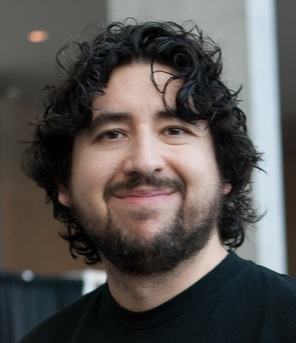
\includegraphics[width=2.08333in,height=\textheight]{images/John_Gruber,_2009_(cropped) - By Randy Stewart, CC BY-SA 3.0, httpscommons.wikimedia.orgwindex.phpcurid=10682505.jpg}\end{minipage}%

\end{figure}%

He aquí uno de los grande valores que busca el movimiento en favor de
una \emph{ciencia abierta}: \textbf{romper las barreras que limitan el
acceso a los textos y a los datos}. El uso de \emph{texto plano} para
escribir y organizar archivos de datos tienen muchas ventajas. Para
empezar se pueden leer prácticamente en cualquier dispositivo,
independientemente de \emph{sistema operativo} e intereses comerciales
de los fabricantes. Los archivos escritos así han superado la \emph{dura
prueba del paso del tiempo} mejor que otros tipos de archivos.

El día de hoy empezaremos a utilizar la idea del \emph{Markdown}.
Producirás tus primeros archivos que serán legibles como texto plano y
que a la vez estarán listos para ser producidos en una variedad de
presentaciones que usualmente requerimos para nuestro propio registro de
actividades y para interactuar con colegas o maestros. Además, de lo que
hizo en su momento \emph{Gruber}, ahora existen herramientas como
\textbf{Pandoc}, que pueden convertir archivos desde \emph{Markdown} a
una variedad de otros formatos que seguramente serán de tu interés en
algún momento. Otro de los valores de la \emph{ciencia abierta}:
\textbf{favorecer el reuso de los productos de información y
conocimiento}

\subsection{Quarto}\label{quarto}

Lo que haremos es:

\begin{enumerate}
\def\labelenumi{\arabic{enumi}.}
\tightlist
\item
  Arrancar \emph{RStudio}
\item
  Crear un nuevo proyecto
\item
  {!!!Empezar a escribir!!!}
\end{enumerate}

\emph{Rstudio} tiene en su menu \textbf{file} la opción de preparar
documentos en \emph{Quarto}.

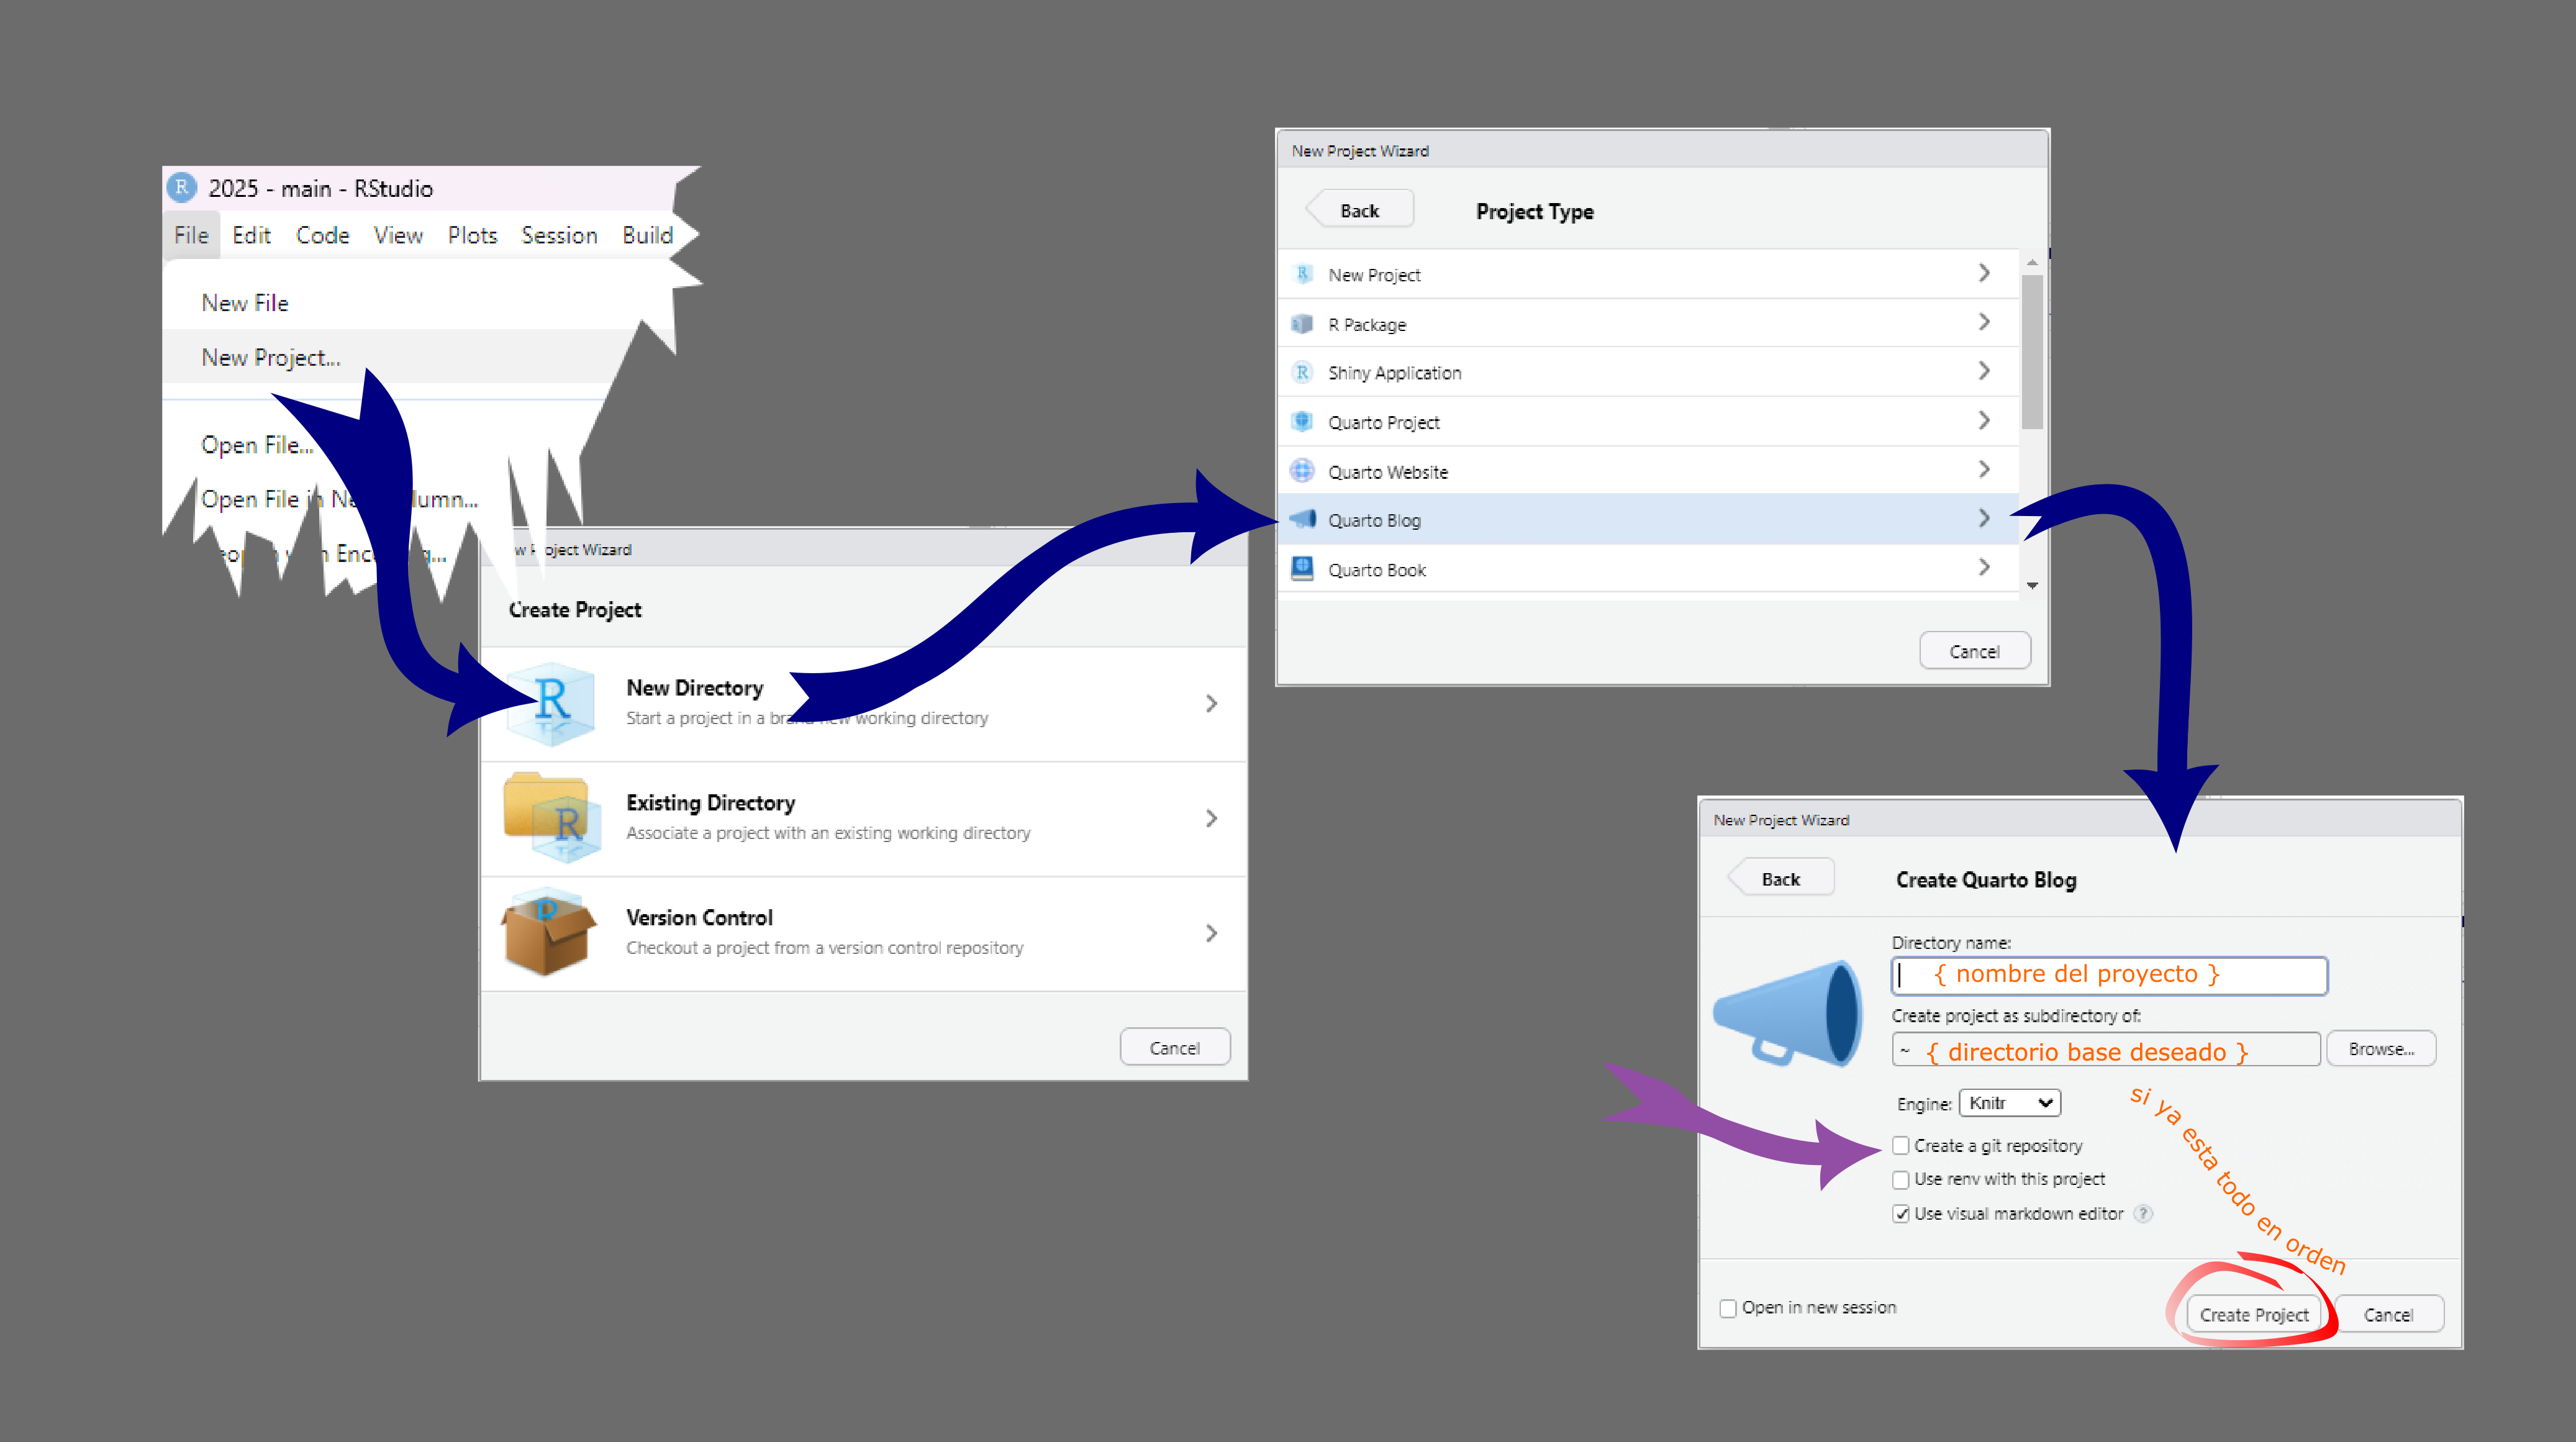
\includegraphics{images/proyecto-blog.png}

\subsection{Guardar con la intención de
colaborar}\label{guardar-con-la-intenciuxf3n-de-colaborar}

Ahora ya tenemos el texto en nuestras máquinas, almacenado en casa.
¿Podemos hacer algo más para asegurar esos materiales y facilitar
compartirlos con quienes queramos? Te sugiero considerar \textbf{git} y
\textbf{github} para eso. Podemos imaginar que el espacio de
almacenamiento en tu máquina es como una parcela de siembra, cada dato
tiene coordenadas de localización y así los recuperas cuando los
quieres. Lo que hace \emph{git} es agregar una \emph{ventana de tiempo}
que te permite asomarte a la historia de lo que pasó en esas ubicaciones
que te interesan.

\begin{figure}[H]

\caption{Fuente: \emph{Final.doc} en \textbf{Piled Higher and Deeper}
por Jorge Cham, http://www.phdcomics.com}

{\centering 
\includegraphics[width=0.6\textwidth,height=\textheight]{images/version_control_motivation_comics.png}

}

\end{figure}%

\subsubsection{¿Qué es Git?}\label{quuxe9-es-git}

Es una aplicación diseñada por el iniciador del desarrollo de Linux
\href{https://es.wikipedia.org/wiki/Linus_Torvalds}{Linus Torvalds}.
\href{https://git-scm.com/}{Git} es un sistema eficiente confiable y
distribuido de control de versiones. El control de versiones es
simplemente el seguimiento y registro de los cambios que va teniendo un
documento a lo largo del tiempo. El concepto \emph{distribuido} se
refiere a que el registro local que tengas en tu máquina o para el caso
en cualquier número de máquinas, es un registro completo,
\textbf{clonado} del proyecto. Estos repositorios locales plenamente
funcionales permiten trabajar aún cuando no tengas acceso a Internet.
Los autores realizan y registran su trabajo localmente y, cuando lo
encuentren conveniente, sincronizan la copia local del repositorio con
la del servidor. En la actualidad \emph{Git} se ha convertido en el
estándar mundial \emph{de facto} para el control de versiones.

Para activar \textbf{git} en tu proyecto tienes dos opciones:

\begin{enumerate}
\def\labelenumi{\arabic{enumi}.}
\tightlist
\item
  Hacerlo desde el principio marcando la casilla respectiva al momento
  de crear el proyecto.
\item
  Utilizar la biblioteca de herramientas auxiliares
  \href{https://usethis.r-lib.org/articles/git-credentials.html}{\texttt{usethis}}.
\end{enumerate}

Con este comando creas lo necesario para usar \textbf{git} en tu
proyecto.

\begin{Shaded}
\begin{Highlighting}[]
\NormalTok{usethis}\SpecialCharTok{::}\FunctionTok{use\_git}\NormalTok{()}
\end{Highlighting}
\end{Shaded}

En cualquier caso, ahora conviene verificar como está configurado el
espacio de trabajo. En la ventana de \textbf{consola} puedes escribir
los siguientes comandos para averiguar detalles de tu configuración.

Esto te dirá como se llama la \emph{ventana de tiempo} que has elegido
definir como base de trabajo, puedes tener tantas ramas distintas como
consideres, pero conviene que una sea la principal. Se solía llamar a
esta rama \textbf{master}, pero ahora se ha considerado que la
!esclavitud ya ha sido abolida!, así que hay una tendencia a mejor
llamarle \textbf{main}. En realidad puedes llamarla como quieras.

\begin{Shaded}
\begin{Highlighting}[]
\NormalTok{usethis}\SpecialCharTok{::}\FunctionTok{git\_default\_branch}\NormalTok{()}
\end{Highlighting}
\end{Shaded}

Si quieres configurar tu instalación de \textbf{RStudio} para que
siempre defina la rama base como \emph{main}, puedes usar elsiguiente
comando. Aunque esto sólo actuará para futuros proyectos, no cambiará
nada en los que tienes ya creados hasta este momento.

\begin{Shaded}
\begin{Highlighting}[]
\NormalTok{usethis}\SpecialCharTok{::}\FunctionTok{git\_default\_branch\_configure}\NormalTok{(}\AttributeTok{name =} \StringTok{"main"}\NormalTok{)}
\end{Highlighting}
\end{Shaded}

Si lo que quieres es modificar la rama principal del proyecto con el que
estas trabajando y que ya tienes abierto, este es el comando que te
ayudará. En este ejemplo uso lo que es ya práctica común, migrar de
\emph{master} a \emph{main}, pero puedes tomar tus propias preferencias
sin ningún problema, aunque obviamente la parte \textbf{from} debe ser
la existente que deseas modificar.

\begin{Shaded}
\begin{Highlighting}[]
\NormalTok{usethis}\SpecialCharTok{::}\FunctionTok{git\_default\_branch\_rename}\NormalTok{(}\AttributeTok{from =} \StringTok{"master"}\NormalTok{, }\AttributeTok{to =} \StringTok{"main"}\NormalTok{)}
\end{Highlighting}
\end{Shaded}

No todos los archivos que están en el espacio de trabajo son realmente
de interés como para seguir su historia en el tiempo y podría haber
también cosas que nunca deberían estar registradas en un sistema que te
expone al acceso público generalizado: claves personales, tokens,
identificadores de archivos privados, etc. Aunque ante esto no hay mejor
cosa que ser prudente y estar atentos, existe la función
\texttt{vacunar} que busca ayudarte a evitar estos problemas. Para
activar esta ayuda en tu proyecto puedes usar este comando.

\begin{Shaded}
\begin{Highlighting}[]
\NormalTok{usethis}\SpecialCharTok{::}\FunctionTok{git\_vaccinate}\NormalTok{()}
\end{Highlighting}
\end{Shaded}

Esto pone ya en operación las capacidades de \textbf{git} en tu máquina.
Para usarlas debes dirigirte a la pestaña respectiva. Con la función
\textbf{Commit} generas el registro del estado de los archivos del
proyecto al momento de activar el comando. Para operar esto debes
decidir que archivos enviar al registro histórico, marcados como
\emph{staged}. Al apretar el botón \textbf{Commit} aparecerá una ventana
en donde se reportan los detalles de lo que estas registrando. Cada
\textbf{Commit} requiere anotar un mensaje descriptivo breve de lo que
contiene el ``corte''. Una vez que está todo resuelto, hay que apretar
el botón \textbf{Commit} en esa pantalla y esperar algunos segundos a
que termine el proceso de registro en la base de datos respectiva.

\subsection{\texorpdfstring{Enviar el \emph{repositorio} \textbf{git} a
la
nube}{Enviar el repositorio git a la nube}}\label{enviar-el-repositorio-git-a-la-nube}

Ahora estas preparada o preparado para enviar tu trabajo a \emph{la
nube}, lo haremos con el servicio de \textbf{Github}, aunque hay varias
opciones (como \textbf{gitlab} por ejemplo).

Nuevamente nos ayudará \texttt{usethis}para hacer esto. Lo primero es
que para comunicar \textbf{RStudio} con \textbf{Github} necesitas
registrar un \textbf{token} de ese servicio en tu equipo. El comando
para esto es:

\begin{Shaded}
\begin{Highlighting}[]
\NormalTok{usethis}\SpecialCharTok{::}\FunctionTok{create\_github\_token}\NormalTok{()}
\end{Highlighting}
\end{Shaded}

Esto te lleva a la página de \textbf{Github} en la que hay que generar
el \textbf{token}. Hay que responder las preguntas que te haga la
página, aunque todo estará \emph{prellenado} con lo normalmente
necesario. Cuando esté a tu gusto, aprieta el botón respectivo.
Aparecerá una nueva pantalla con el \textbf{token} que habrá que copiar
al \emph{portapapeles} (\textbf{ctr-c} en Windows). Este \textbf{token}
que aparece, es la única vez que lo verás, por lo que conviene copiarlo
al \emph{portapapeles} de tu máquina (\textbf{ctrl-c} en windows) y
tenerlo a buen resguardo por lo pronto. En seguida hay que ejecutar este
otro comando en la consola de \emph{RStudio}

\begin{Shaded}
\begin{Highlighting}[]
\NormalTok{gitcreds}\SpecialCharTok{::}\FunctionTok{gitcreds\_set}\NormalTok{()}
\end{Highlighting}
\end{Shaded}

Si es la primeta vez que registras un \textbf{token} te pedirá que lo
registres, dale \emph{paste} (\textbf{ctrl-v} en Windows). Si ya tienes
un registro dado de alta, te informará sobre lo que tiene anotado y te
dará oportunidad de decidir qué quieres hacer en seguida.

Todo está ya preparado, sólo falta poner en uso el vínculo que acabamos
de crear. Para eso bastará con decir:

\begin{Shaded}
\begin{Highlighting}[]
\NormalTok{usethis}\SpecialCharTok{::}\FunctionTok{use\_github}\NormalTok{()}
\end{Highlighting}
\end{Shaded}

Por cierto, este es el comando qe necesitarán en lo sucesivo para
vincular cualquier nuevo proyecto a tt centta ed \textbf{Github},
siempre y cuando tu \textbf{token} este vigente.

\begin{figure}

\begin{minipage}{0.67\linewidth}
Una vez teminadas estas tarea puedes ir a la pestaña \textbf{git} cuando
lo consideres conveniente y ordenar a \textbf{RStudio} que envié todos
los \textbf{commits} que están pendientes hasta el momento a
\textbf{Github}. Para hacerlo deberás apretar el botón \textbf{Push}.
Antes de hacerlo siempre es conveniente pedirle a \textbf{git} que se
ponga al día con lo que ya está registrado en la \emph{nube}, esto lo
logras con el botón \textbf{pull}. Esto nos lleva a una rutina de
operación con \textbf{git} que se resume en la figura
siguiente.\end{minipage}%
%
\begin{minipage}{0.33\linewidth}
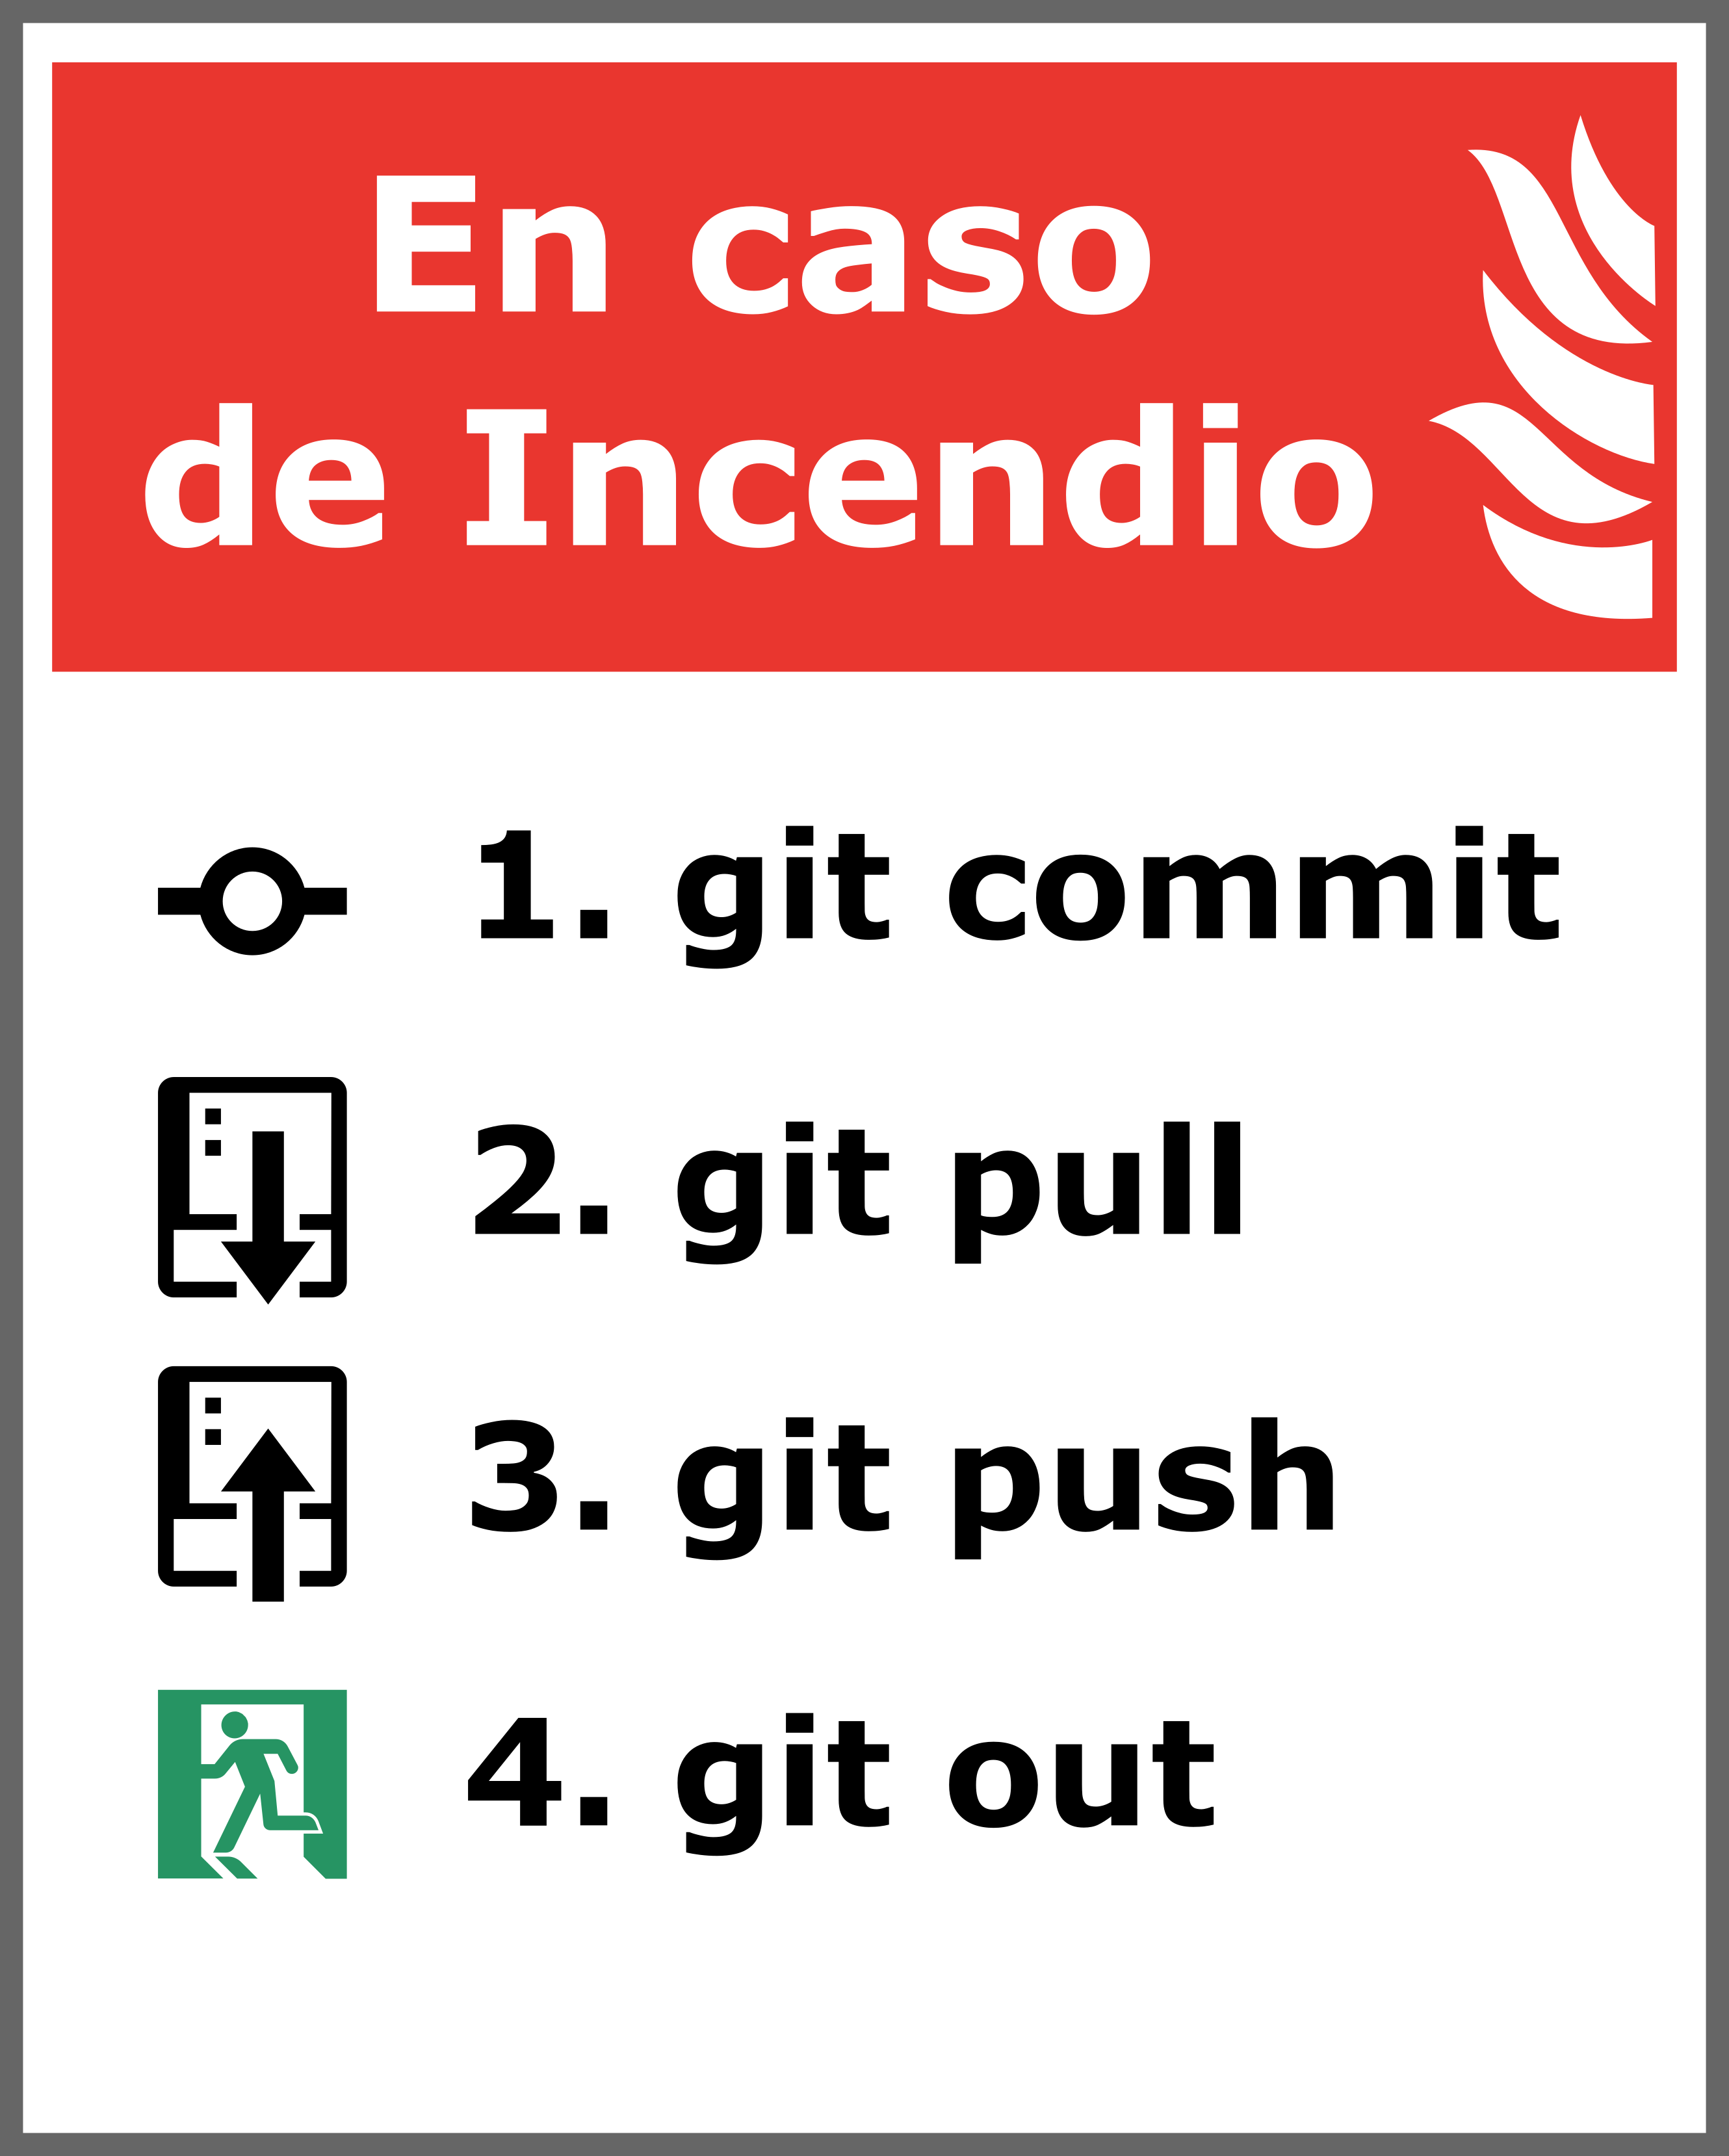
\includegraphics[width=1.5625in,height=\textheight]{images/En caso de incendio.png}\end{minipage}%

\end{figure}%

\subsubsection{\texorpdfstring{Resumen rutinario para usar
\textbf{git}}{Resumen rutinario para usar git}}\label{resumen-rutinario-para-usar-git}

Claro está que configurar todo la primera vez es un poco complicado,
pero si todo está listo: git instalado, cuenta de Github, token
activado, etc. la operación cotidiana es mucho más sencilla.

En la figura se ilustran las dos rutas para hacerlo en \emph{RStudio}.

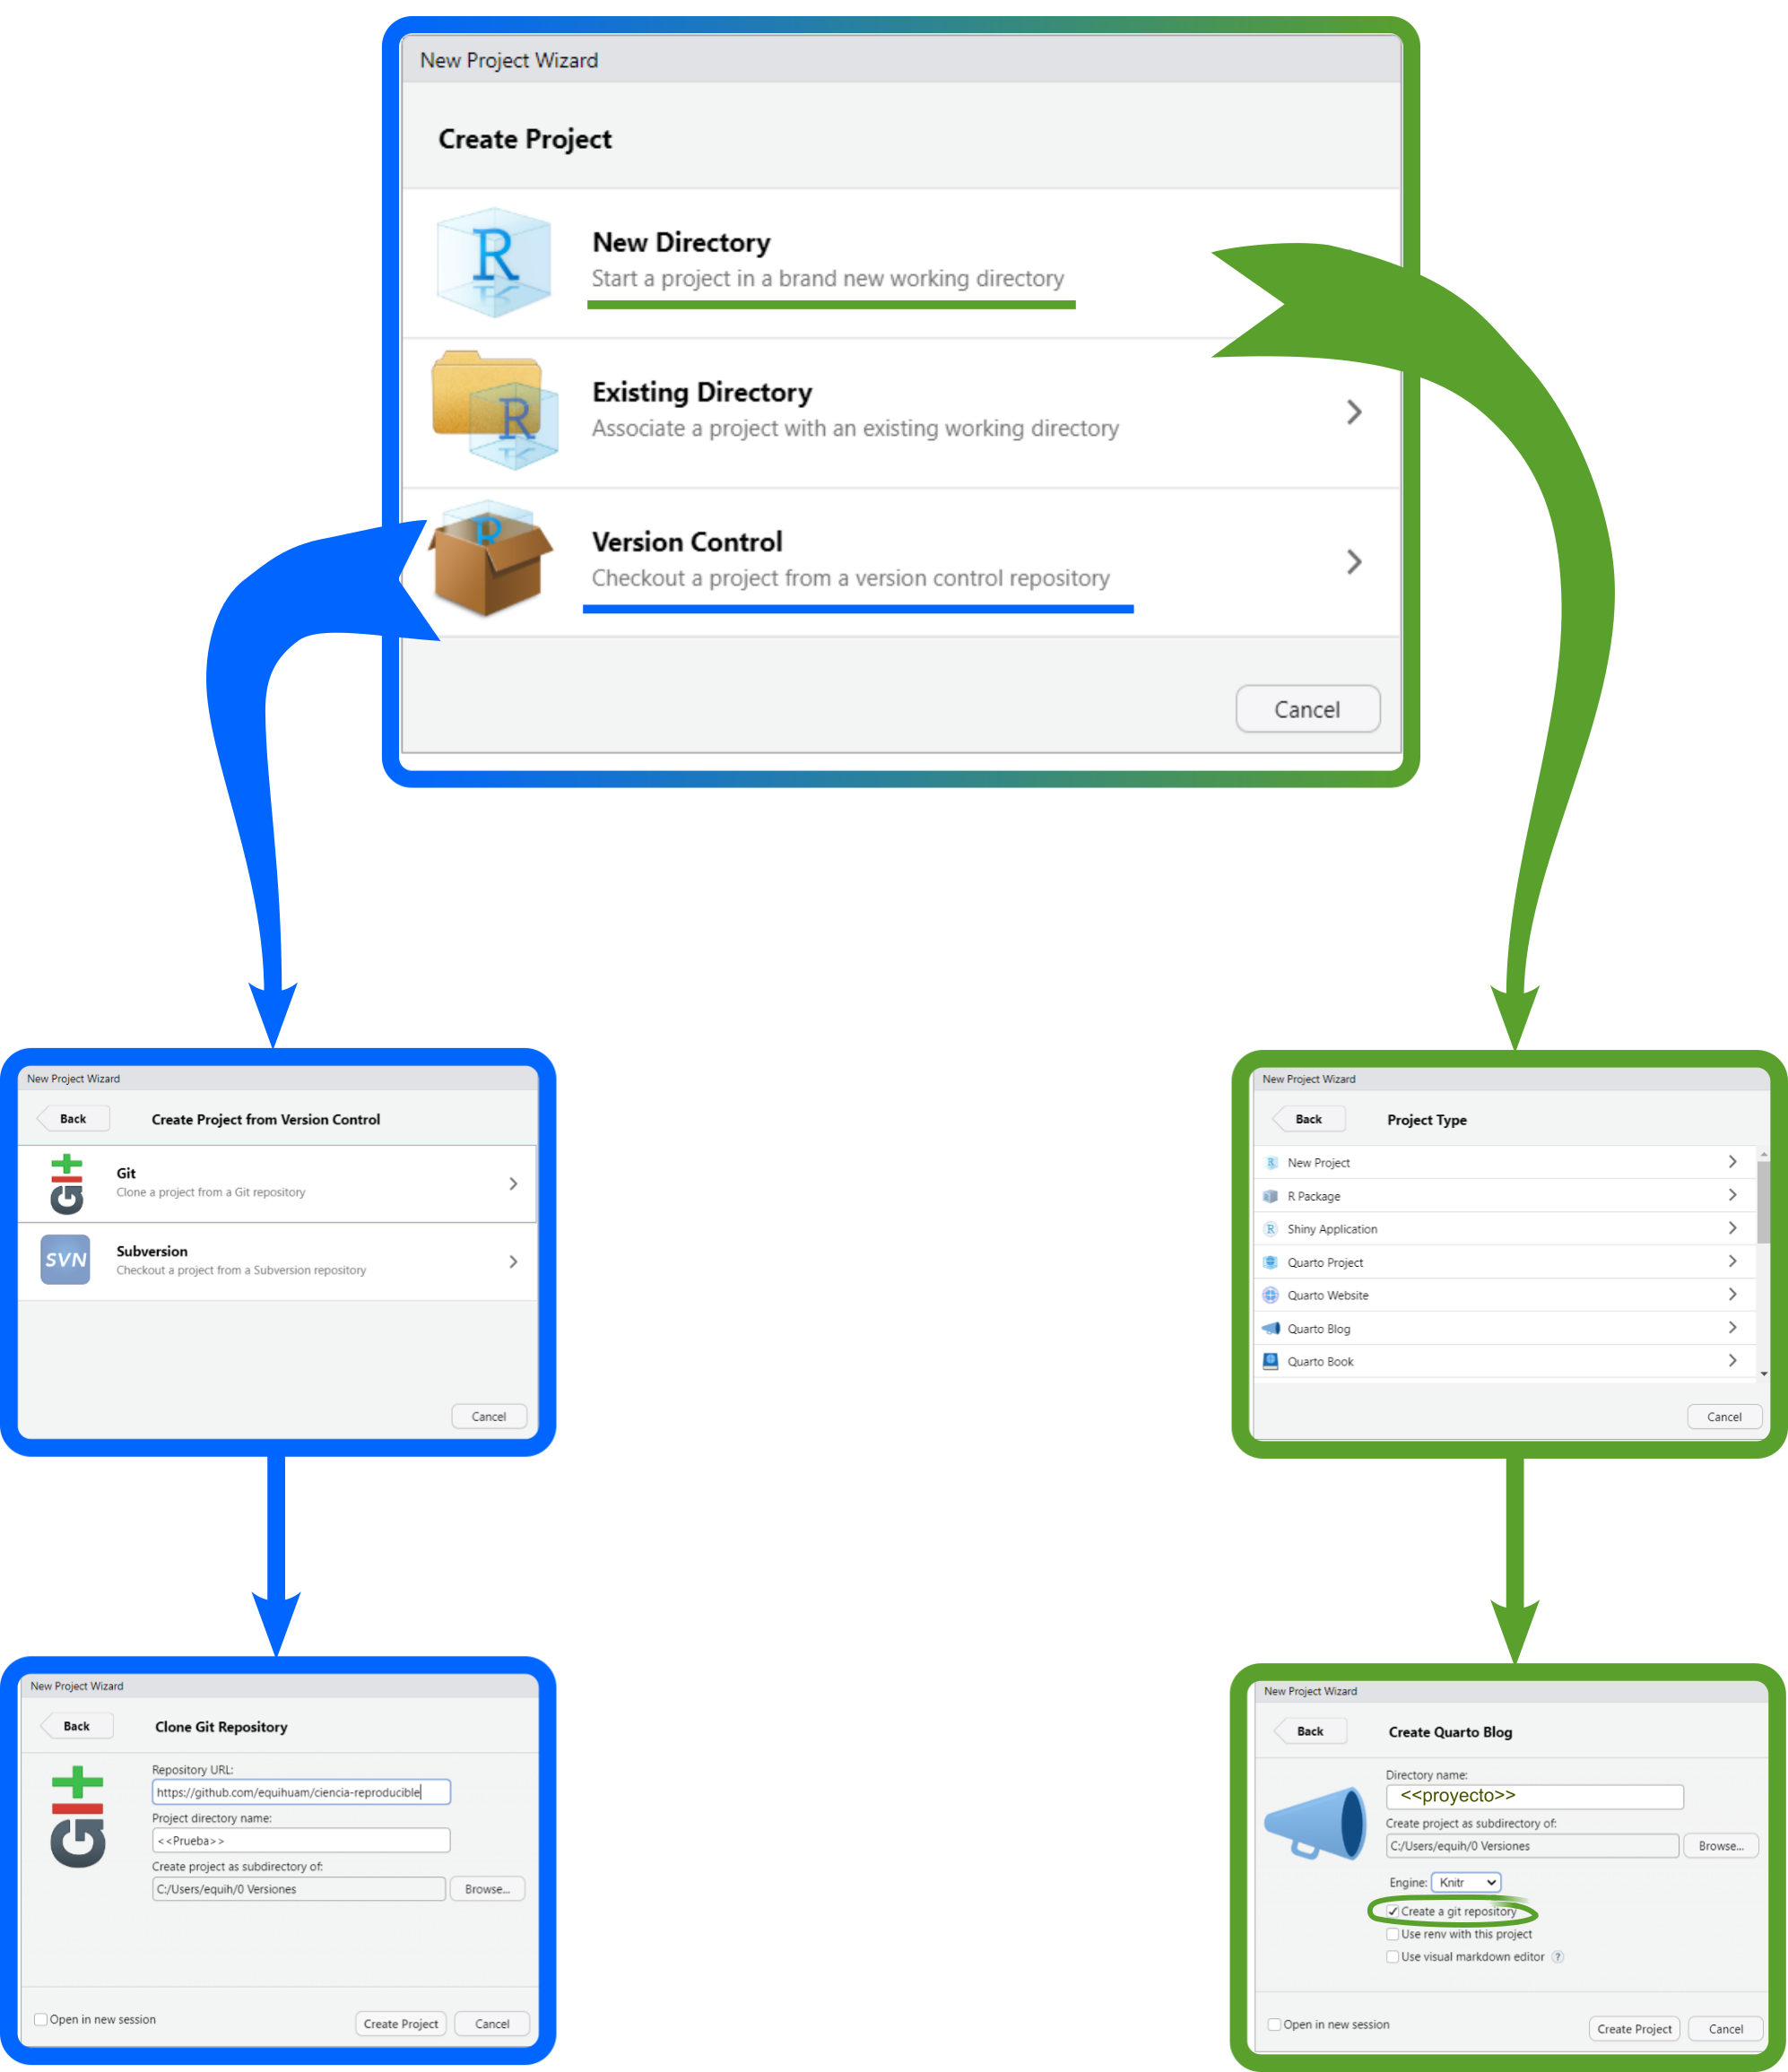
\includegraphics{images/proyecto-con-git.png}

Evidentemete, si seguiste la ruta azul, tu repositorio ya existe en
\emph{Github}, una vez qe hayas \textbf{clonado} el repositorio en t
máquina todo queda listo para concentrarte en escriibir. Si optaste por
la ruta verde, entonces deberás crear un nuevo repositorio en
\emph{Github}. Para hacerlo Utiliza \texttt{usethis} en la pestaña de
consola.

\begin{Shaded}
\begin{Highlighting}[]
\NormalTok{usethis}\SpecialCharTok{::}\FunctionTok{use\_github}\NormalTok{()}
\end{Highlighting}
\end{Shaded}

Eso es todo.

\hfill\break

\subsection{Asociar Github con Netlify para publicar tu
Blog}\label{asociar-github-con-netlify-para-publicar-tu-blog}

Hay que preparar a \emph{Github} dando acceso a \emph{Netlify} para que
tome lo necesario. La meta es que construya un sitio Web con tu
contenido y lo publique en Internet. Los pasos que hay que seguir para
esta primera interacción son los siguiente.

Iniciar la vinculación con Github seleccionando la opción que ofrece
importar los documentos desde un \emph{repo} Git. Esto dará la opción de
utilizar \emph{Github} como origen de datos, entre otras posibilidades.

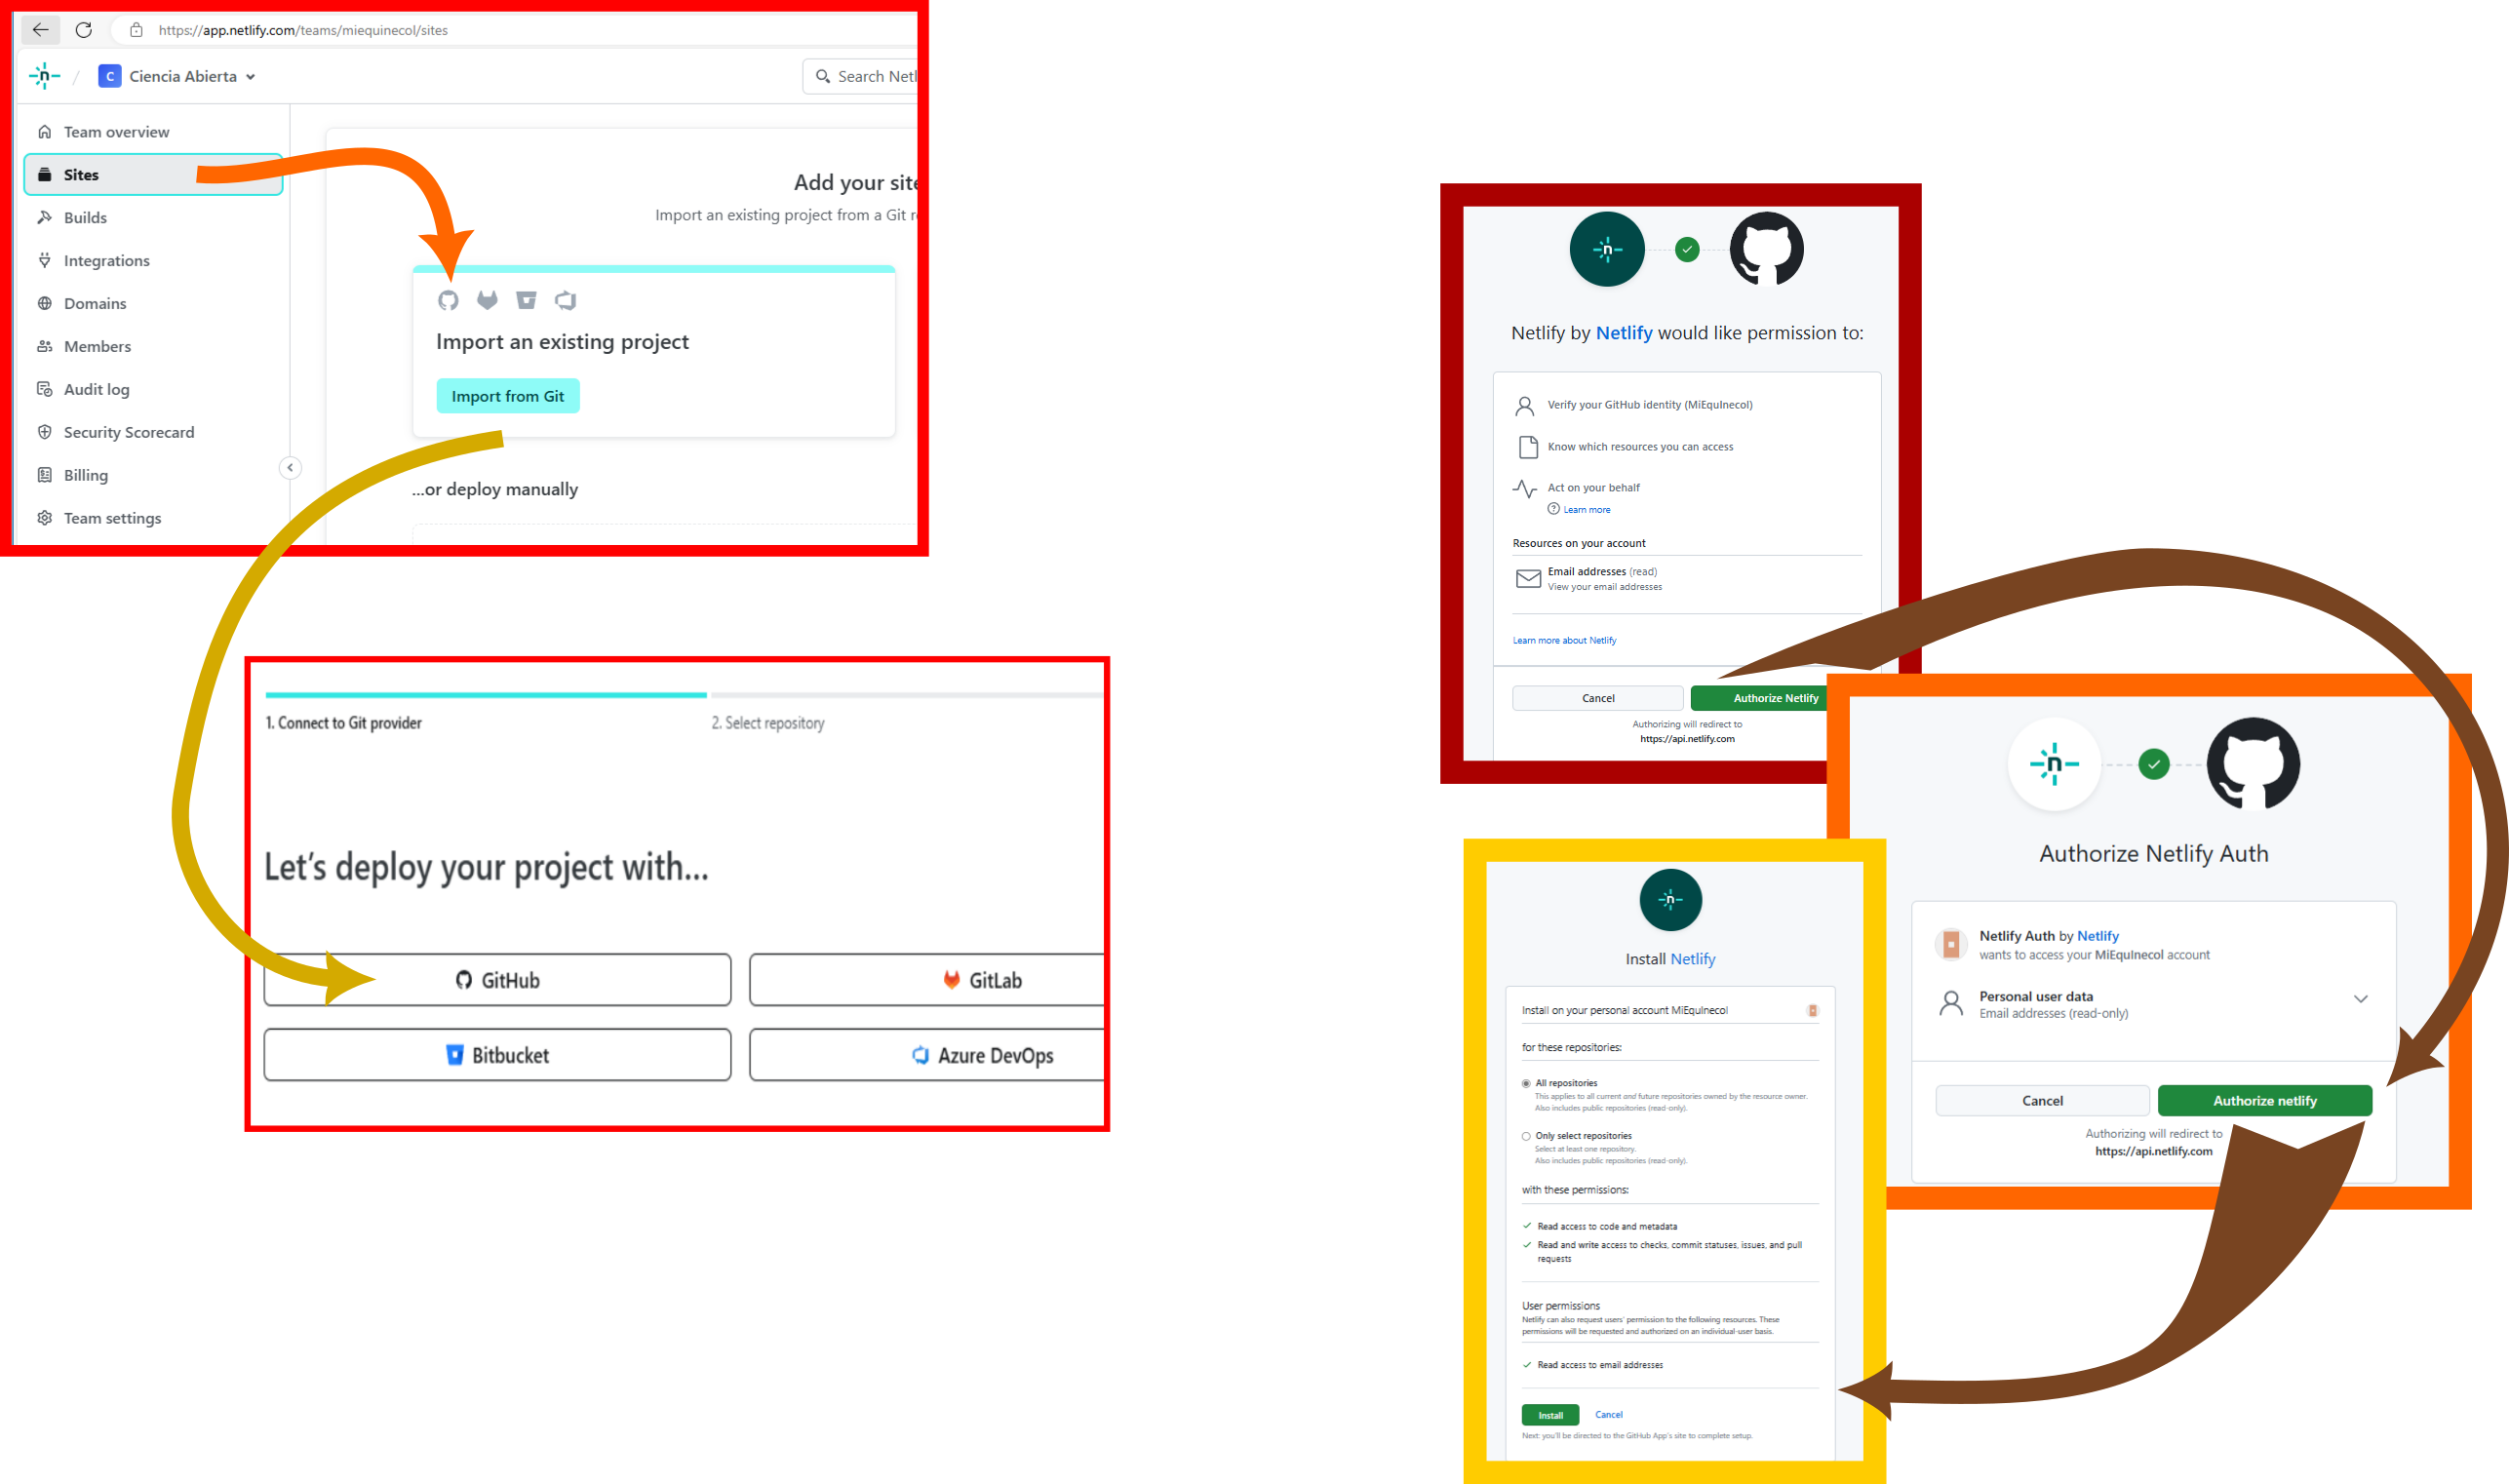
\includegraphics{images/Netlify-1.png}

El Siguiente paso es autorizar a Netlify a acceder a Github a través de
tu cuenta, así como los específicos del repositorio que te interesa
vincular. Esto también implica instalar una \textbf{aplicación} de
vínculo entre \emph{Netlify} y \emph{Github} dentro de tu cuenta.

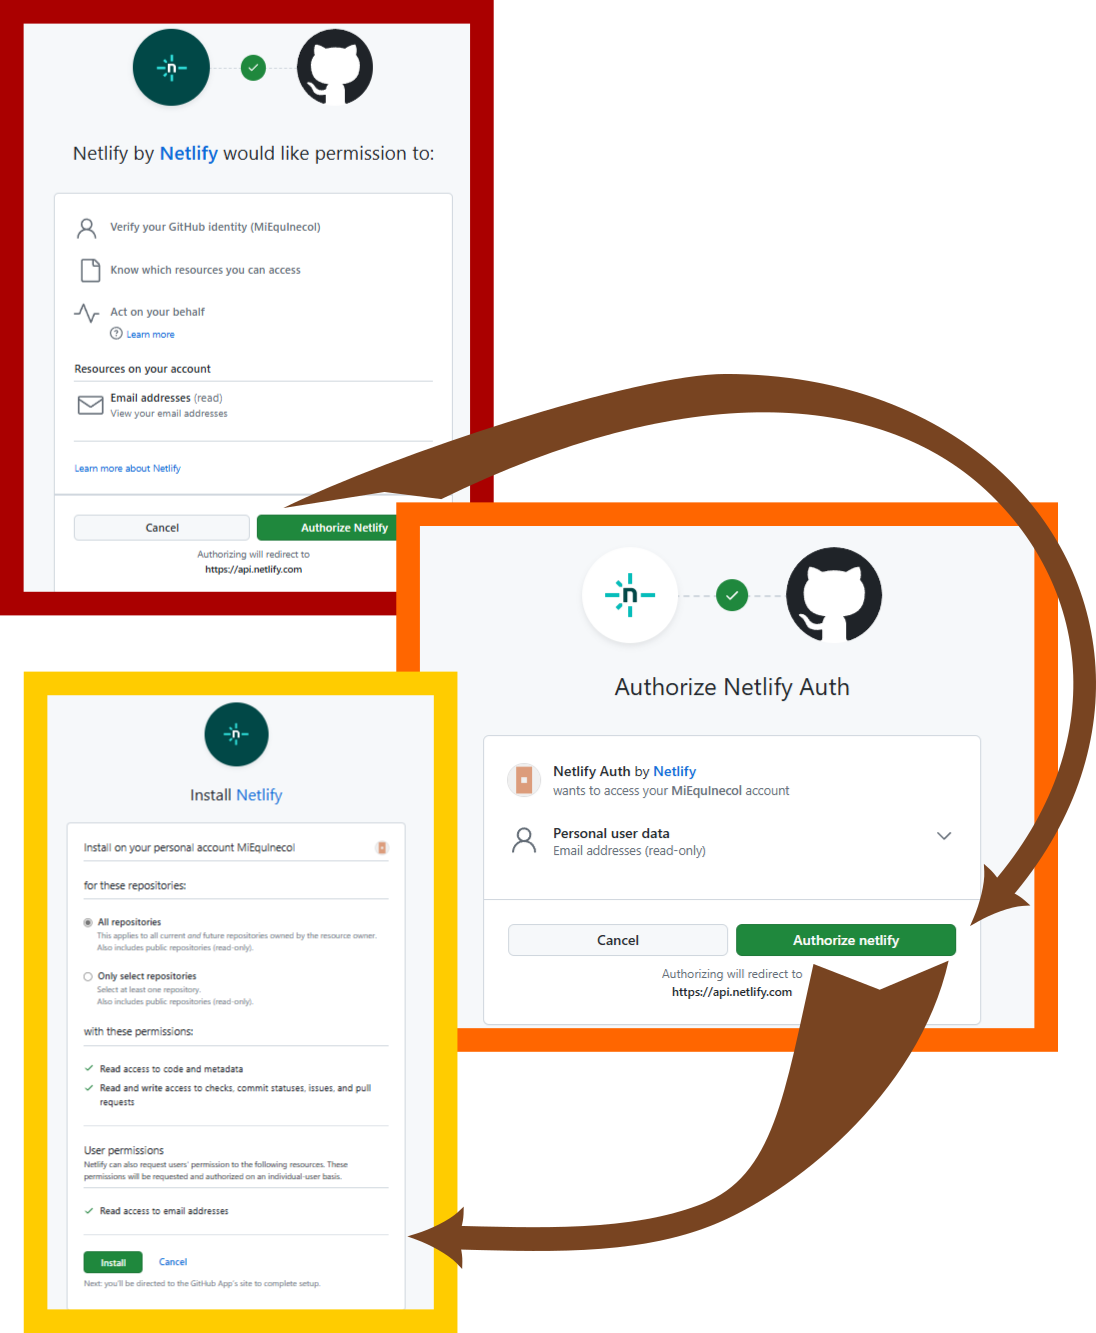
\includegraphics{images/Netlify-2.png}

Si todo ocurrió sin problemas, tendrás ahora en \emph{Github}, en el
menú de aplicaciones (Avatar→ Settings→ Applications), un botón que te
permitirá configurar el vínculo con \emph{Netlify} según tus
requerimientos. También podrás ver los \emph{repos} que hayas autorizado
desde \emph{Netlify}.

\subsection{Creación de un nuevo sitio a
publicar}\label{creaciuxf3n-de-un-nuevo-sitio-a-publicar}

\begin{enumerate}
\def\labelenumi{\arabic{enumi}.}
\item
  \textbf{En Netlify}:

  \begin{itemize}
  \tightlist
  \item
    Desde la opción \emph{team} o \emph{site} puedes generar un nuevo
    sitio.
  \end{itemize}
\end{enumerate}

\begin{figure}

\begin{minipage}{0.50\linewidth}
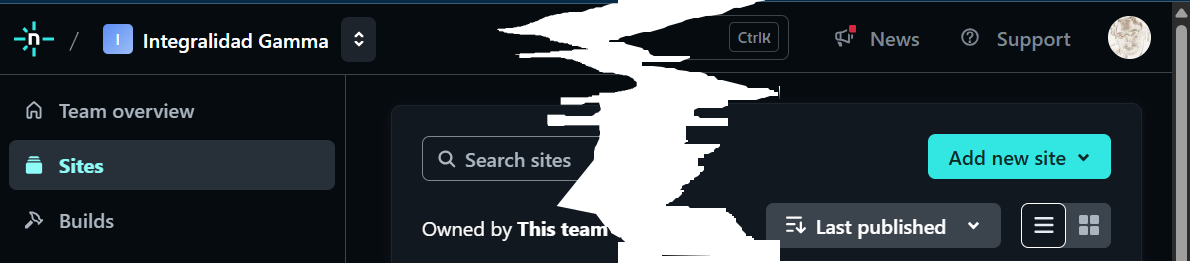
\includegraphics{images/Netlify-new-site.png}\end{minipage}%
%
\begin{minipage}{0.50\linewidth}
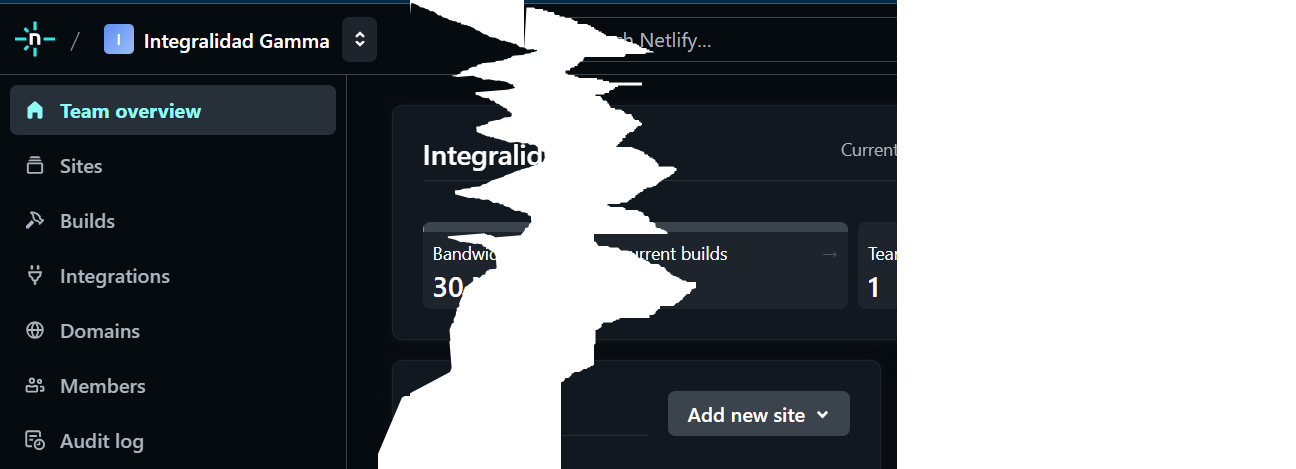
\includegraphics{images/Netlify-new-site-team.png}\end{minipage}%

\end{figure}%

Cuando aprietas el boton de \emph{añadir sitio}, aparecerá una nueva
pantalla que tiene tres secciones. Se trata de los atributos que tendrás
que proporcionar para darle presencia en Internet a tu proyecto y
algunos otros atributos que definen como se producirá y actualizará
continuamente. Estas operaciones es poco probable que las vuelvas a ver,
una vez que tu proyecto esté en producción, aunque desde luego estarán
siempre ahí por si deseas hacer ajustes.

\paragraph{¿Qué nombre le daras?}\label{quuxe9-nombre-le-daras}

Deberás elegir un nombre que se convertirá en una URL para acceder a tu
proyecto. Puede ser cualquier cosa que desees, pero debe ser único. En
esta sección puedes escribir nombres y verificar que estén disponibles

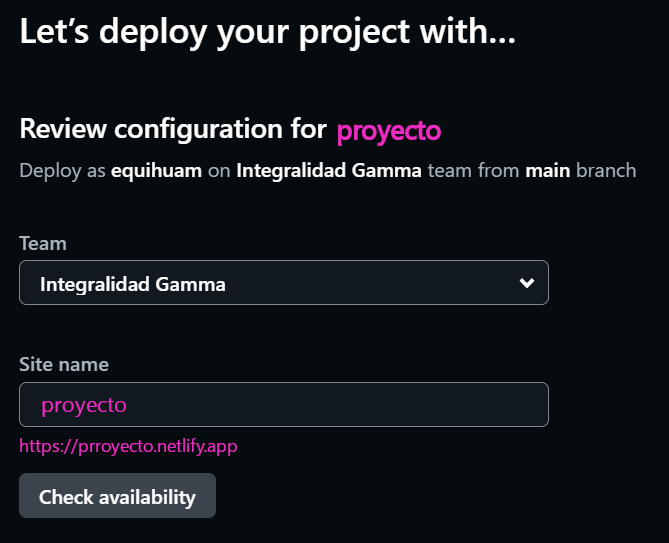
\includegraphics[width=0.5\textwidth,height=\textheight]{images/Netlify-config-site-1.png}

\paragraph{¿Qué hará Netlify para operar tu
sitio?}\label{quuxe9-haruxe1-netlify-para-operar-tu-sitio}

Es una colección de atributos para indicarle a \emph{Netlify} dónde
conseguir los documentos y como manejarlos. En nuestro caso, muy simple,
básicamente hay que decirle en donde están los documentos que
\emph{Quarto}, con ayuda de \emph{pandoc}, ha \emph{renderizado}. Si no
has cambiado nada en \texttt{\_quarto.yml} la rama que estamos usando
aquí para que \emph{Git} los registre es \textbf{main} y, en ella el
directorio de producción se llama **\_site**. Por favor verifica el
contenido de esto para ayudarte a comprender mejor lo que estás
haciendo.

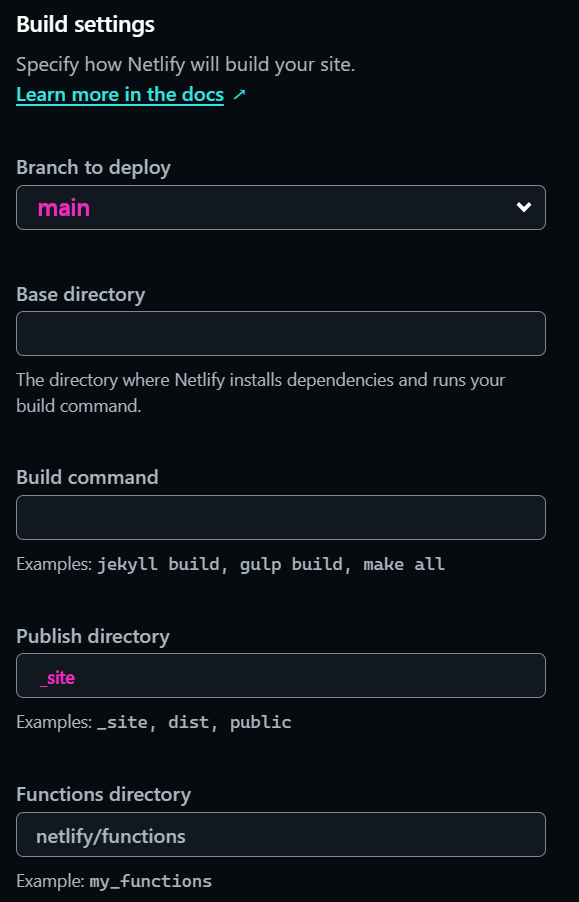
\includegraphics[width=0.5\textwidth,height=\textheight]{images/Netlify-config-site-2.png}

\paragraph{¿Todo listo? ¡a
producción!}\label{todo-listo-a-producciuxf3n}

En nuestro caso no hay más que hacer, \emph{Netlify} tiene información
suficiente para encargarse de publicar tu proyecto continuamente.
Incorporará los cambios que hagas en \emph{RStudio} en la rama
principal. Lo hará automáticamente cada vez que envíes tus cambios a
\emph{Github}.

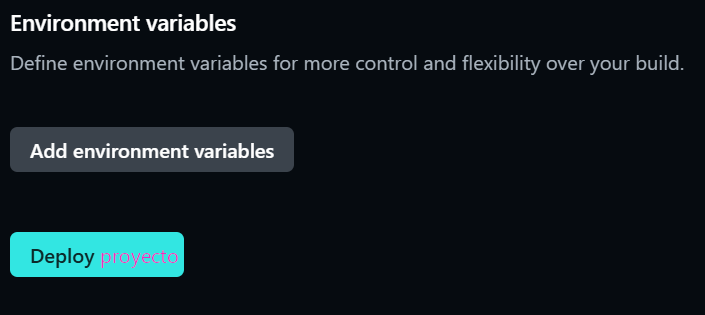
\includegraphics[width=0.5\textwidth,height=\textheight]{images/Netlify-config-site-3.png}

Si todo salió bien, en este momento ya debe estar tu proyecto publicado
y accesible para cualquier lector del mundo que lo localice y se
interese en su contenido.

\begin{tcolorbox}[enhanced jigsaw, colbacktitle=quarto-callout-tip-color!10!white, bottomtitle=1mm, opacityback=0, leftrule=.75mm, toprule=.15mm, arc=.35mm, breakable, coltitle=black, colframe=quarto-callout-tip-color-frame, colback=white, opacitybacktitle=0.6, toptitle=1mm, titlerule=0mm, title=\textcolor{quarto-callout-tip-color}{\faLightbulb}\hspace{0.5em}{Finalmente ¿Cómo quedá todo organizado?}, rightrule=.15mm, bottomrule=.15mm, left=2mm]

\begin{enumerate}
\def\labelenumi{\arabic{enumi}.}
\tightlist
\item
  Tienes un proyecto en tu máquina
\item
  Está vinculado con tu cuenta en \textbf{Github}
\item
  Están vinculados \textbf{Github} y \textbf{Netlify}
\end{enumerate}

Ahora, sólo queda crear el contenido del Blog. Recuerda usar un
directorio para cada nueva contribución dentro de la carpeta
\emph{posts}. Te sugiero usar un esquema \emph{fecha-tema} para llamar
esos archivos. Evita usar espacios y caracteres latinos en esos temas.
Para trabajar hay que crear un archivo \emph{index.qmd}. Puedes hacerlo
desde el menu: \emph{File} \$ \$ \emph{New Quarto document\ldots{}}

Configura el encabezaddo de control con algo así como:

\begin{Shaded}
\begin{Highlighting}[]
\CommentTok{{-}{-}{-}}
\AnnotationTok{title:}\CommentTok{ "Los primeros pasos"}
\AnnotationTok{author:}\CommentTok{ "Miguel Equihua"}
\AnnotationTok{lang:}\CommentTok{ es}
\AnnotationTok{date:}\CommentTok{ 21/feb/2025}
\AnnotationTok{categories:}\CommentTok{ [taller, inicio, markdown, rstudio, git]}
\AnnotationTok{image:}\CommentTok{ "images/Image by Mojca{-}Peter from Pixabay {-} seeds{-}1217133\_1280.jpg"}
\AnnotationTok{code{-}fold:}\CommentTok{ true}
\AnnotationTok{code{-}summary:}\CommentTok{ "muestra el escript:"}
\AnnotationTok{fig{-}cap{-}location:}\CommentTok{ top}
\CommentTok{{-}{-}{-}}
\end{Highlighting}
\end{Shaded}

Si es de tu interés, aquí encontrarás
\href{https://rpubs.com/drgregmartin/1266674}{muchos detalles
interesanes sobre YAML}

\end{tcolorbox}



\end{document}
